%%*************************************************************************
%%
%% Anomaly Detection by Means of Statistical Analysis of the Frequency Spectrum
%% V1.1
%% 2011/12/22
%% by Peter Boraros
%% See http://www.pborky.sk/contact for current contact information.
%%
%%*************************************************************************
%%
%% Legal Notice:
%%
%% This code is offered as-is without any warranty either expressed or
%% implied; without even the implied warranty of MERCHANTABILITY or
%% FITNESS FOR A PARTICULAR PURPOSE! 
%% User assumes all risk.
%%
%% This work by Peter Boraros is licensed under a 
%% Creative Commons Attribution-NonCommercial-ShareAlike 3.0 Unported License.
%% http://creativecommons.org/licenses/by-nc-sa/3.0/
%%
%%*************************************************************************

\documentclass[a4paper,journal]{IEEEtran}

\usepackage{cite}
% \usepackage[nocompress]{cite}
\usepackage{ifpdf}

\ifpdf
\usepackage[pdftex]{graphicx}
\graphicspath{{./img/}}
\DeclareGraphicsExtensions{.pdf}
\else
\usepackage[dvips]{graphicx}
\graphicspath{{./img/}}
\DeclareGraphicsExtensions{.eps}
\fi

\usepackage[cmex10]{amsmath}
\usepackage{amsfonts}
\usepackage{amssymb}
\interdisplaylinepenalty=2500

\usepackage{algorithmic}

\usepackage{array}

\usepackage{mdwmath}
\usepackage{mdwtab}

\usepackage{eqparbox}

\usepackage[hang,small,center,bf]{caption}
% \usepackage[tight,normalsize,sf,SF]{subfigure}
%\usepackage[tight,footnotesize]{subfigure}
\usepackage{subfig}
% \usepackage[caption=false,font=normalsize,labelfont=sf,textfont=sf]{subfig}
% \usepackage[caption=false,font=footnotesize]{subfig}

\usepackage[utf8x]{inputenc}
\usepackage{url}
\usepackage{fixltx2e}
\usepackage{stfloats}
\usepackage{ucs}
\usepackage{multirow}

% correct bad hyphenation here
\hyphenation{op-tical net-works semi-conduc-tor}

\renewcommand{\labelitemi}{$\bullet$}
\renewcommand{\labelitemii}{$\circ$}
\renewcommand{\labelitemiii}{$\ast$}

\setlength{\textheight}{260mm}

\begin{document}

\title{Anomaly Detection by Means of Statistical Analysis of the Frequency Spectrum}
\date{July 25, 2011}
\author{Peter~Boráros %
\thanks{{Peter Boráros}, Czech technical university, Faculty of Electrical Engineering,
see~\texttt{http://www.pborky.sk/contact} for a contact infomation}}%

% The paper headers
%\markboth{Peter Boráros, Czech technical university, Faculty of Electrical Engineering, Prague, Czech Republic}{}

\IEEEcompsoctitleabstractindextext{%
\begin{abstract}
This article provides information about statistical analysis of the frequency spectrum of a computer network traffic.
The computer network traffic can be seen as an sequence of events occuring in time domain. This ought to be 
transformed to the frequency domain and then a statistical model of particular behaviors ought to be found. 
The model is then usable to statistical inference and recognition of some security problems in computer network.
\end{abstract}}

\maketitle
\IEEEdisplaynotcompsoctitleabstractindextext
\IEEEpeerreviewmaketitle

\section{Introduction}\label{sec1}
Motivation for this work is to enable ability to distinguish a periodic behavior of potential threats from ordinary
network communication. Dataset that has been provided for purposes of this work contains an agregate information of 
about one day of the network communication as well as the information of malignancy of particular communication 
participants. The crucial moment of this research is to differentiate an malicious peer-to-peer communication from
other not-malicous classes (especially www proxy servers or DNS servers).

Section \ref{sec:prep} provides formal information about data capturing, and process of extracting features involving 
fourier transformation. In section \ref{sec:stats} an usage of the statistical methods is described and in section 
\ref{sec:exp} is described the aplication on given dataset. 
Especially the construction and verification of the statistical models. 

Reader interested in statistical analysis should skip to section \ref{sec:stats}. 

\section{Data preparation}\label{sec:prep}
\subsection{Network traffic, gathering the data}
It is possible to represent a network traffic by set of flows distributed in time. The flow is a sequence of packets having  similar attributes. Packets are exchanged usually among network endpoints. Attributes taken under consideration are at least: source and destination endpoint address, port and protocol. Mentioned attributes usualy delimitate flows.

In order to evaluate anomaly rate of paticular flow other properties ought to be taken in account. Especially number of packets and bytes, starting and ending time (time-stamp of the first or the last packet in the flow).

%TODO mention the features 
The time distribution of flows can be determined by considering the starting timestamp of each flow. This approach provides generalized view on the flow, as it has been occured in network channel with unlimited throughput.

Experimental dataset provided for purposes of this work has been extended with classification information, a knowledge if particular endpoint is harmfull or not or even if it is suspicious.

\subsection{Data binning}
In order to reduce minor observation errors binning technique ought to be used. The time axis is divided into disjoint intervals - bins. Let $h$ be number of bins and $\mathbb{F}$ be the set of all flows captured in time interval $\mathbb{T} = (0, T_{max}\rangle $. The $t$-th bin is known as  set of flows $\mathbb{F}_t$ that occurs in time interval $\mathbb{T}_t = ((t-1)\cdot \delta, t\cdot \delta\rangle $ where $t \in \{1, .. h\}$ and $\delta$ is the width of time intervals denoted $\delta = \frac{T_{max}}{h}$. Denote
\begin{equation}
\mathbb{F}_t = \{f : f \in \mathbb{F} \wedge s(f) \in \mathbb{T}_t \}
\end{equation}
where function $s:\mathbb{F} \rightarrow \mathbb{N} $ 
returns starting timestamp of the flow $f\in \mathbb{F}$.

For each interval,
representative value is calculated. Following formulas have been considered:
\begin{equation}
r_t^{(1)} = \frac{\sum\limits_{f\in \mathbb{F}_t}b(f)}{\sum\limits_{f\in \mathbb{F}_t}p(f)}
\end{equation}
\begin{equation}
r_t^{(2)} = \log(1+\sum\limits_{f\in \mathbb{F}_t}p(f))
\end{equation}
where $r_t$ is representative of time interval $t$, $\mathbb{F}_t$ is set of flows captured in time 
interval $t$, function $b:\mathbb{F} \rightarrow \mathbb{N}$ outputs size of the flow $f$ in bytes and function 
$p:\mathbb{F} \rightarrow \mathbb{N}$ outputs the packet count of the flow $f$.

%TODO further description of representatives and features

\subsection{Fourier transformation}
Representatives $r_t$ are subject to transformation from the time domain to the
frequency domain.
This can be achieved by fourier-related
tranforms, e.g. by a fourier or a wavelet transform.
The wavelet transform, unlike the fourier transform, captures
not only a notion of the frequency content of the input, by
examining it at different scales, but also temporal content.

To achieve fast computation, a fast fourier transform (FFT) algorithm 
has been involved.
It is an efficient algorithm to compute the discrete fourier tranform (DFT) and
its inverse.
A DFT decomposes a sequence of values into components of
different frequencies. 
This operation is useful in many fields but computing it directly from the
definition is often too slow to be practical.
An FFT is a way to compute the same result more quickly: 
computing a DFT of N points in the naive way, using the definition, takes
$O(N^2$) arithmetical operations, 
while an FFT can compute the same result in only $ O(N \log N)$ operations.

The sequence of $N$ complex numbers $x_0, ..., x_{N−1}$ is transformed into the
sequence of $N$ complex numbers $X_0, ..., X_{N−1}$ by the DFT according to the
formula:
\begin{equation}
X_k = \sum_{n=0}^{N-1} x_n e^{-\frac{2 \pi i}{N} k n} \quad \quad k = 0, \dots, N-1
\end{equation}
where $i$ is imaginary unit and $e^{-\frac{2 \pi i}{N} k n}$ is $N$-th root of
unity. 

The transform is sometimes denoted as 
$\mathcal{F}\colon\mathbb{C}^N \to \mathbb{C}^N$, e.g.
$\mathbf{X} = \mathcal{F} \left ( \mathbf{x} \right )$.

Before processing the fourier transform, the sequence of representatives 
$r_1, ...,r_h$ is choped into overlaping slices.
Each slice (sequence $r_a, ..., r_b$, where $a$ and $b$ are boundaries
of particular slice) is then transformed by means of fourier transformation,
resulting in sequence of complex coeficients for each slice.
By discarding phase information real coeficients ${R}_i$ are obtained,
where $i = 0, ..., b-a-1$.

Slices are ordered as they are occuring in time and they ought to be numbered
$j = 1,..., g $. The count of slices  depends on the number of elements 
in input sequence $h$, on the slice size $w$ and the step size $s$; one of the
$g=\lfloor\frac{h-w}{s} \rfloor$ or $g=\lceil\frac{h-w}{s} \rceil$.
For the sake of convenience the slice size $w$ is power of two.
Let $a_j$ and $b_j$ be the boundaries of the $j$-th slice. Then
$a_1 = 1$, $b_j = a_j + w$ and $a_{j+1} = a_j + s +1$.
For the overlaping slices inequality $s < w$ is valid.

Let $\mathcal{R}$ be matrix of fourier coeficients where
$\mathcal{R}_{i,j}$ is $i$-th fourier coeficient of $j$-th slice,
i.e. 
\begin{equation}
\mathcal{R}_{*,j} = abs(\mathcal{F}(r_{a_j}, ..., r_{b_j}))
\end{equation}
The column vector $\vec R_j = \mathcal{R}_{*,j}$ represents one sample. 
Assuming that the components $r_i$ are independent and identically distributed (i.i.d.) random variables
and declaring $ s \ge w $ (so the slices are not overlaping) also vectors $\vec{R}_j$ are i.i.d.

\subsection{Distinguishing the endpoints}
As mentioned above experimental dataset contains also
classification information pointing out an level of anomaly of 
particular endpoints. Endpoint is determined by its address.
We now extend the definitions mentioned
former in order to be able to distinct the fourier coeficients for
particular endpoint.

Let $\mathbb{E}$ be a set of all endpoints that
participate in coummunication within time interval $\mathbb{T}$.
Let $\mathbb{F}_{t,u \rightarrow}$ be the set of flows captured in
time interval $\mathbb{T}_{t}$ %TODO: refer
which are \textbf{initiated} by the endpoint $u \in \mathbb{E}$,
similarly $\mathbb{F}_{t, \rightarrow u}$ are \textbf{ended} at the
endpoint $u$. Formaly

\begin{equation}
\mathbb{F}_{t,u \rightarrow} = \{f : f \in \mathbb{F} \wedge e_{s}(f) = u \wedge s(f) \in \mathbb{T}_t \}
\end{equation}
\begin{equation}
\mathbb{F}_{t, \rightarrow u} = \{f : f \in \mathbb{F} \wedge e_{d}(f) = u \wedge s(f) \in \mathbb{T}_t \}
\end{equation}
where $e_{s}:\mathbb{F}\rightarrow \mathbb{E}$ and
$e_{d}:\mathbb{F}\rightarrow \mathbb{E}$ 
are functions returning source and destination endpoint for the 
flow $f$.
The representative value of particular bin for particular endpoint is 
then:
\begin{equation}\label{bigrepr1}
r_{t,e}^{(1)} = \frac{\sum\limits_{f\in \mathbb{F}_{t,e}}b(f)}{\sum\limits_{f\in \mathbb{F}_{t,e}}p(f)}
\end{equation}
\begin{equation}\label{bigrepr2}
r_{t,e}^{(2)} = \log(1+\sum\limits_{f\in \mathbb{F}_{t,e}}p(f))
\end{equation}
where index ${}_e$ is replaces symbols ${}_{u\rightarrow}$ or 
${}_{\rightarrow u}$ from previous definition. So it is distinguished 
if the connection is initiated by the endpoint $u$, or ended at the
endpoint $u$.

Matrix of fourier coeficients $\mathcal{R}^\bullet$ is 3-dimensional:
\begin{equation}\label{bigmatrix}
\mathcal{R}^\bullet_{*,j,e} = abs(\mathcal{F}(r_{a_j,e}, ..., r_{b_j,e}))
\end{equation}
First dimension is related to the frequency domain, second to the time domain 
(this is the trend of the fourier coeficients over time), 
and third dimension is related to the endpoint.
We can denote that matrix $\mathcal{R}^{(1)\bullet}$ (resp. $\mathcal{R}^{(2)\bullet}$)
is using representative $r_{t,*}^{(1)}$ (resp. $r_{t,*}^{(2)}$) based on formulas
(\ref{bigrepr1}) and (\ref{bigrepr2}).

\section{Statistical analysis}\label{sec:stats}
In previous section an matrix $\mathcal{R}$, that represents sample set, has been introduced.
Columns of the matrix are $N$-dimensional random vectors that have to undergo further analysis.

At first step, the model (along with the model`s parameters $\theta$) ought to be found.
Most popular methods are based on maximum likelihood estimation (MLE) where the solution is sought by 
iterative manner maximizing the likelihood estimate and iteratively modifying the parameters $\theta$ so the likelihood
estimate increases. An Expectation-Maximization (EM) algorithm is example of such process. It is very popular in 
examining mixture models due to its speed. In \cite{Bor04} it has been shown that this algorithm converges 
to local optima. First question is, if the locally optimal model is good enough. The other question is how accuratelly 
the fitting process approximates the observed distribution even if it finds an global optima.

These reasonable doubts are implying that the parameters obtained by EM algorithm have to undergo a goodness-of-fit
testing by method indepedent from the MLE.
An articles \cite{Nar03}, \cite{Ros62} sugests that for multivariate distribution ($N > 1$) little research
has been accomplished and there is no such universal method like $\chi^2$-test or  Kolmogorov-Smirnov test
for the univariate case ($N=1$). 


\subsection{The model}
In last subsection the process of fittng the model`s parameters have been outlined without any closer look at the model.
Hence, nearer look on the model have to be taken.

Generally, the sample set represented by matrix  $\mathcal{R}$ is the set of $N$-dimensional real vectors.
Denote the $i$-th sample as $\vec{R}_i = (r_{i,1},\ldots,r_{i,N})^T \in  \mathbb{R}^N$.
For $N=1$ it reduces to scalar value $R_i = r_{i} \in  \mathbb{R} $.

Vector $\vec{R}$ can be seen as random vector with unknown probability distribution
$F_R: \mathbb{R}^N \rightarrow \langle 0, 1 \rangle $. Distribution $F_R$ represents the supected model.

There can be doubts about normality of the distribution, but for the sake of convenience a plausible assumption of 
normality of the distribution $F_R$  ought to be verified. Under this assuption the sample set is modelled by multivariate 
normal distribution, denote $\vec{R} \sim \mathcal{N}(\vec{\mu},\mathbf \Sigma)$, where the parameters of the model are 
$\theta = (\vec{\mu}, \mathbf\Sigma)$, $\vec{\mu}$ is mean vector, and $\mathbf\Sigma$ is the covariance matrix. 
Instead of cumulative distribution function $F_R$ we denote an probabilty density function $f_R$:
\begin{equation}
f_R(\vec{\mathbf{t}})\, =
\frac{1}{(2\pi)^{N/2}|\mathbf\Sigma|^{1/2}}
\exp \left(-\frac{1}{2}({\mathbf{\vec t}}-{\mathbf{\vec\mu}})^T{\mathbf\Sigma}^{-1}({\mathbf{\vec t}}-\mathbf{\vec\mu})
\right).
\end{equation}
In case $N=1$ the distribution is reduced to univariate normal distribution $R \sim N(\mu,\sigma)$, where $\mu$ is 
mean value $\mu = ER$ and $\sigma$ is standard deviation $\sigma = \sqrt{DR} = \sqrt{E[(R - ER)^2] }$ and 
probabilty density function $f_R$ is:
\begin{equation}
f_R(t)\, =
\frac{1}{\sqrt{2\pi}\sigma}
\exp \left(-\frac{(t-\mu)^2}{2\sigma^2}
\right).
\end{equation}
A cumulative distribution function could be expressed as:
\begin{equation}
F_R(x) = \int_{-\infty}^x f(t)\,dt.
\end{equation}

\subsection{Fitting the model`s parameters}
The EM algorithm is an efficient iterative procedure to compute the maximum likelihood estimate (MLE) in the
presence of missing or hidden data. In MLE, we wish to estimate the model parameter(s) for which the observed
data are the most likely.

Each iteration of the Expectation-Maximization (EM) algorithm consists of two processes: 
The E-step, and the M-step. In the expectation, or E-step, the missing data are estimated given the observed 
data and current estimate of the model parameters. 
This is achieved using the conditional expectation, explaining the choice of terminology.
In the M-step, the likelihood function is maximized under the assumption that the missing data are known. 
The estimate of the missing data from the E-step are used in lieu of the actual missing data.

Convergence is assured since the algorithm is guaranteed to increase the likelihood at each iteration.

As has been suggested, EM algorithm is used to searching for model in the presence of missing or hidden data.
For example a fitting an gaussian mixture model can be highlighted. Gaussian mixture model is denoted by
$ Mix_{\mathbf{\vec{c}}}(N(\mu_1,\mathbf{\Sigma_1}),\ldots,N(\mu_k,\mathbf{\Sigma_k})) $ where $k$ denominates a number
of mixture components, vector $\vec{c} = (c_1,\ldots,c_k)^T$ is mixture weight vector and it must sum to 1.
Algortihm fits the mixture model while each component of mixture and the weight vector $\vec{c}$
is hidden property of provided sample data (for example an unspecified clustering).

In this article a closer look on simple gaussian model, has been taken. 
Mixture model is out of scope of this article.

\subsection{Univariate goodness-of-fit test - Anderson-Darling test}
Anderson-Darling test is considered as most powerful statistical tool for detecting most departures from normality. 
\cite{Ste74} Its test statistic is based on empirical distribution function.

The Anderson–Darling test assesses whether a sample comes from a specified distribution. It makes use of the fact that, 
when given a hypothesized underlying distribution and assuming the data does arise from this distribution, 
the data can be transformed to a uniform distribution. 
The transformed sample data can be then tested for uniformity with a distance test (Shapiro 1980).
The formula for the test statistic $A^2$ to assess if data $\{R_1,\ldots,R_n\}$ comes from a distribution with cumulative distribution function (CDF) $F_R$:
\begin{equation}
A^2=-n-\sum_{k=1}^n \frac{2k-1}{n}\left[\ln( F_R(R_k)) + \ln\left(1-F_R(R_{n+1-k})\right)\right].
\end{equation}
Note that data must be put in the order: $\forall i,j = 1,\ldots,n: (i \le j) \implies R_i \le R_j $.

The test statistic can then be compared against the critical values of the theoretical distribution.
Note that in this case no parameters are estimated in relation to the distribution function $F_R$.

In case of testing for the normality $R \sim N(\mu, \sigma)$, with known parameters $\mu$ and $\sigma$, 
the test statistic is
\begin{equation}
A^2=-n-\sum_{k=1}^n \frac{2k-1}{n}\left[\ln( \Phi(T_k)) + \ln\left(1-\Phi(T_{n+1-k})\right)\right],
\end{equation}
where $T_k = \hat\sigma^{-1}(R_k - \hat\mu)$ ($R_k$ standardized), 
$\Phi$ is standard normal cumulative distribution function $N(1,0)$
and  $\hat\mu = \mu$, $\hat\sigma = \sigma$ (if parameters are known). 

If $A^2$ exceeds given critical value hypotesis of normality is rejected with som significance level.
The critical values are given in \textsc{table \ref{tbl:crit}}.

\begin{table}[!h]
\caption{Critical values of the test statistic $A^2$ for the particular significance levels}
\begin{center}
\begin{tabular}{|c|c|}\hline
\textbf{Significance} & $\mathbf{A^2_{max}}$ \\ \hline
15\% & 0.576 \\ \hline
10\% & 0.656 \\ \hline
5\% & 0.787 \\ \hline
2.5\% & 0.918 \\ \hline
1\% & 1.092 \\ \hline
\end{tabular}
\end{center}
\label{tbl:crit}
\end{table}
\subsection{Multivariate goodness-of-fit test}
Unfortunately in multivariate case, hypotesis testing is much more complicated. \textsc{Rosenblatt} \cite{Ros62} suggests 
mapping the set of all $N$-dimensional distributions in a one to one measurable manner into a subset of one-dimensional
distribution functions. An \cite{Bro08} brings a closer look on the Rosenblatt`s transformation and its generalization.

Article \cite{BicBre83} suggest using an volume of nearest neighbour sphere centered an particular point of tested dataset.
In \cite{Nar03} multivariate clustering method is introduced.

Multivariate goodness-of-fit tests are out of scope of this article.%, although ..

\section{Experiments}\label{sec:exp}
A set of three matrices  $\{\mathcal{R}^{(1)},\mathcal{R}^{(2)},\mathcal{R}^{(3)}\}$ has been captured and
have to undergo model finding and checking procedure. The upper index $^{(i)}$ distinguishes between three matrices.
An upper index has been omitted, if there is no need to distinguish.

Size of each matrix is $[N \times m]$.
Columns of this matrices contain independent and identically distributed $N$-dimesional random vectors.
For the purposes of this article we \emph{choose} only first dimesion of all \emph{column vectors} to undergo analysis.
Hence we select first row of each of the \emph{matrice} $\mathcal{R}^{(i)}$.
Each component of selected \emph{row} vector is independent and identically distributed random sample.
Analysis of the other dimensions is out of scope of this article.

Denote vectors that undergo analysis as ${\vec R^{(i)}}=( r^{(i)}_1,\ldots,r^{(i)}_{m})$, 
where $i=1,2,3$, and  size of each vector is $m$.

Each of the vectors captures different type of computer network traffic, as shown in the
\textsc{table \ref{tbl:data}}.

\begin{table}[!h]
\caption{Datasets}
\begin{center}
\begin{tabular}{|c|c|c|}\hline
\textbf{No.} & \textbf{Class} & \textbf{Data} \\ \hline
1 & proxy server & $\vec{R}^{(1)}$ \\ \hline
2 & dns server & $\vec{R}^{(2)}$ \\ \hline
3 & p2p network & $\vec{R}^{(3)}$ \\ \hline
\end{tabular}
\end{center}
\label{tbl:data}
\end{table}

Proxy server and DNS server is considered to be legitimate, while p2p network not.

\subsubsection{Model fitting}
Under assumption that given random sample sets are from normal distribution,
the appropiate model have to be found. 
This can be achieved by already introduced EM algorithm, but for normal distribution, 
parameters can be estimated using formulae:
\begin{equation}
\mu = \hat\mu_m = \frac{1}{m}\sum^m_{i=1}r_{i},
\end{equation}
\begin{equation}
\sigma = S_m = \sqrt{\frac{1}{m-1}\sum^m_{i=1}(r_{i}-\hat\mu)^2},
\end{equation}
where $\hat\mu_m$ is mean value of samples, $ S_m$ is sample standard deviation.
\emph{Note} that $\hat\mu_m$ and  $ S_m$ are unbiased estimators of the parameters $\mu$, $\sigma$.
Results are in shown in the \textsc{table \ref{tbl:params}}. The number $m$ is sample set size.
The EM algorithm lead to absolutely same results, even if random initialization has been performed, 
so for simple cases is its usage obsolete.

Cumulative distribution fuctions along with histograms are shown on \textbf{fig. \ref{fig:hist}}.

\begin{figure}[t]%
  \centering
  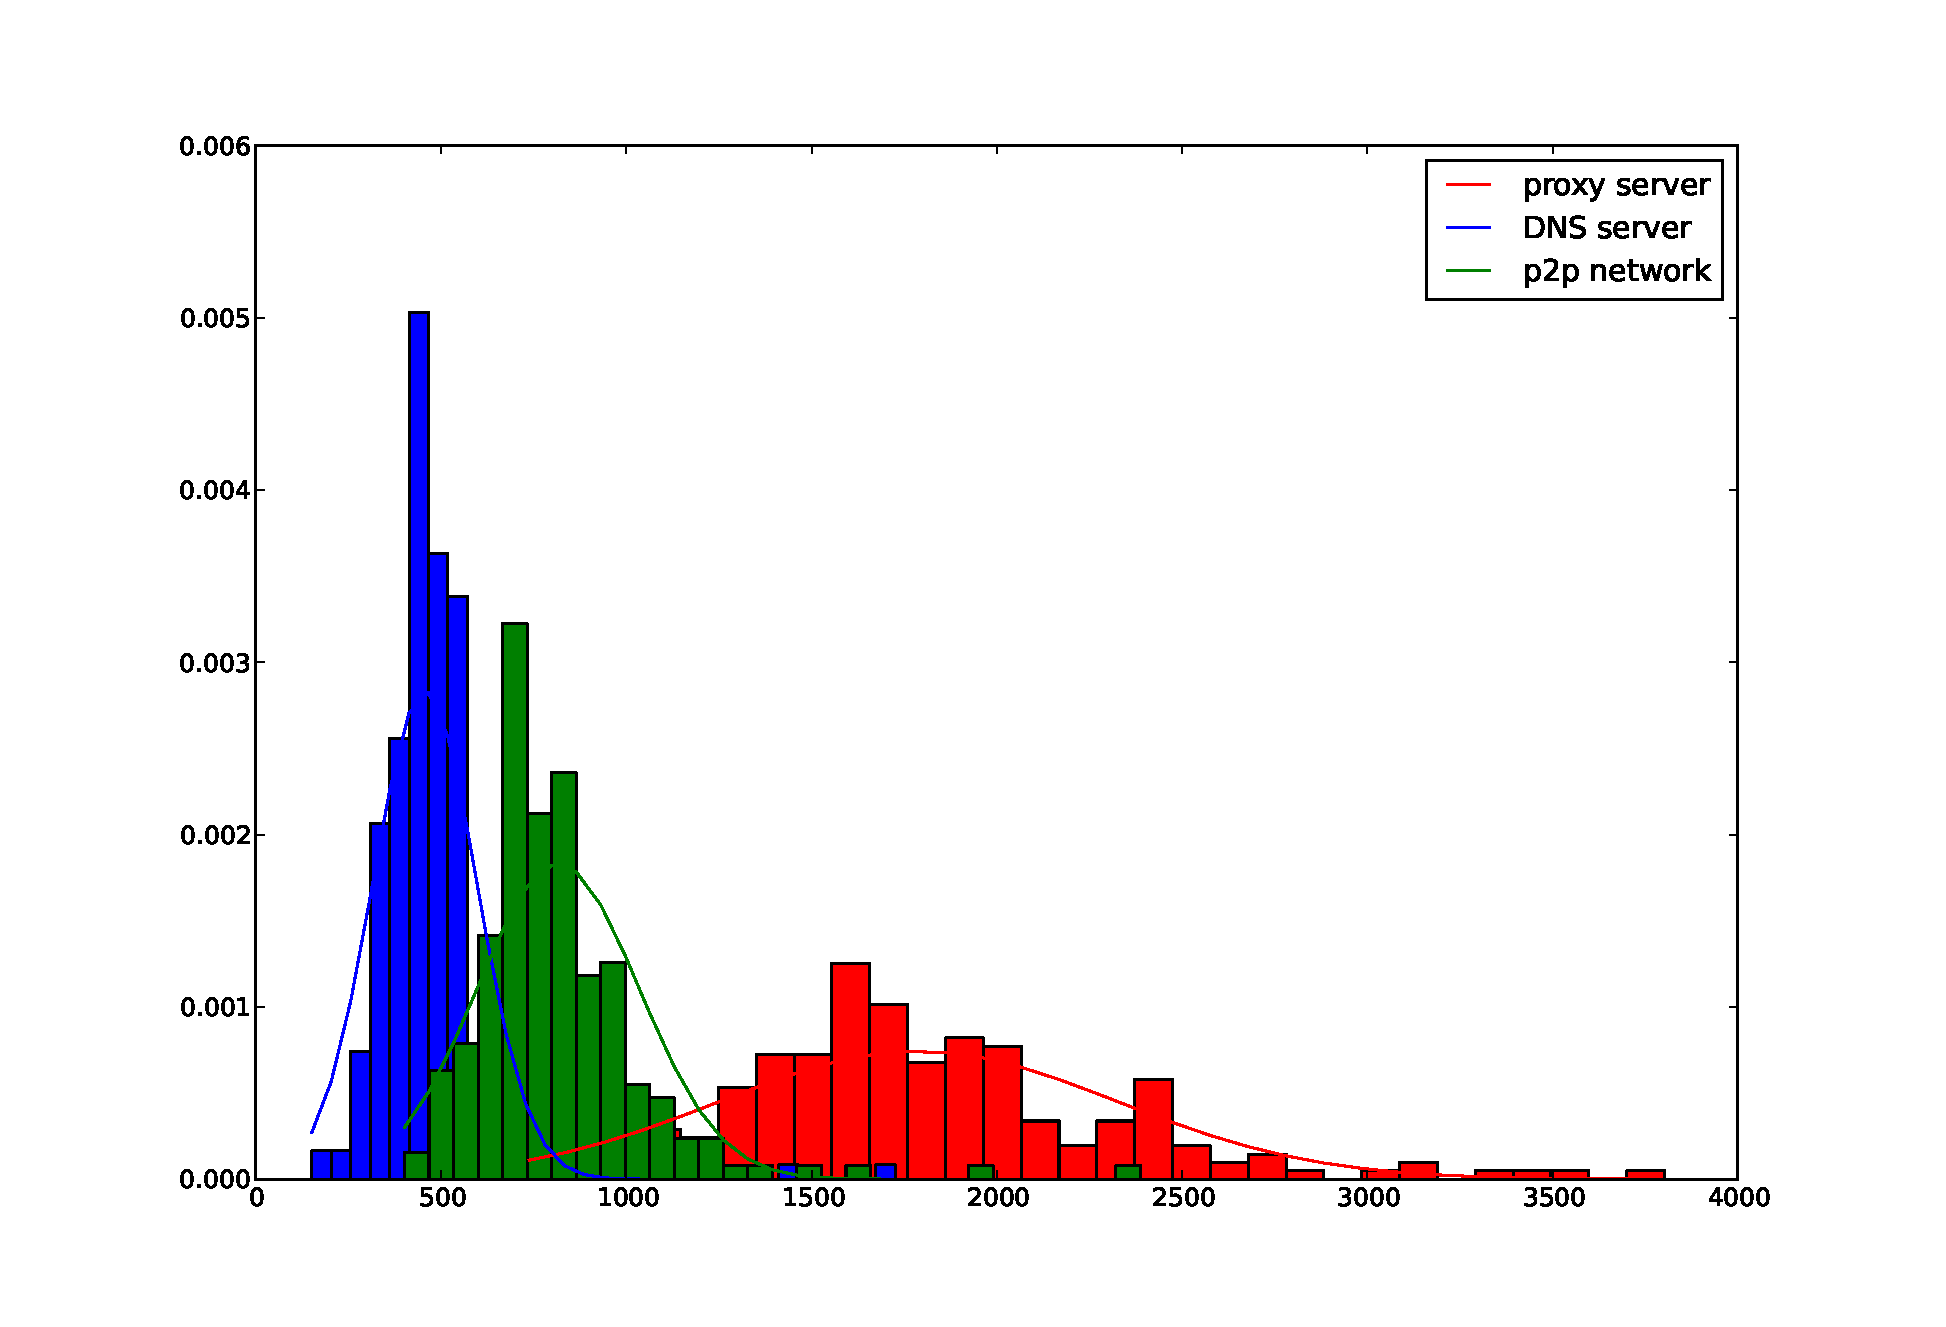
\includegraphics[width=80mm]{hist_gauspdf_dst}
  \caption{Normed histogram and tested probability density function}
  \label{fig:hist}
\end{figure}

\begin{table}[!h]
\caption{Estimated parameters of models}
\begin{center}
\begin{tabular}{|c|c|c|c|c|}\hline
\textbf{No.} & \textbf{Class}  & $\mathbf{\mu_m}$ & $\mathbf{\sigma_m}$ & \textbf{m} \\ \hline
1 & proxy server & 1788.89 & 531.03 & 1870 \\ \hline
2 & dns server & 459.51 & 144.53 & 1867 \\ \hline
3 & p2p network & 812.43 & 212.81  & 1871 \\ \hline
\end{tabular}
\end{center}
\label{tbl:params}
\end{table}

\subsubsection{Goodness-of-fit measure}

The test statistics are in  \textsc{table \ref{tbl:anders}}.
The value $n$ is the number of samples used for test.
\textsc{Stephens} \cite{Ste74} notes that the test becomes better when the parameters 
are computed from the data. Despite of his note different sample set were used to compute the test statistics.
The model has been computed using one set
and the test statistic using other one. 
Anyway, as the statistic exceeds $A^2_{max}$ value, hypotesis of normality can be rejected in all cases
at significance level 1\%.

\begin{table}[!h]
\caption{Test statistics}
\begin{center}
\begin{tabular}{|c|c|c|c|}\hline
\textbf{No.} & \textbf{Class} & $\mathbf{A^2}$ &  \textbf{n} \\ \hline
1 & proxy server & 43908.04 & 200 \\ \hline
2 & dns server & 33334.23 & 203 \\ \hline
3 & p2p network & 58299.30 & 199 \\ \hline
\end{tabular}
\end{center}
\label{tbl:anders}
\end{table}

\section{Conclusion}
Simple experiments described above are not the goal of the research.
Further research of model finding and checking is intended to be done. 
Next experiments will employ gaussian mixture models along with the EM algorithm. 
The goal is, to work out  an easy-to-use and fast method for searching and especially for testing 
 multivariate mixture models.

\begin{thebibliography}{1}

\bibitem{Bor04}
  \textsc{S. Borman}. (2004). \emph{The Expectation Maximization Algorithm - A short tutorial}.
  
\bibitem{Nar03}
  \textsc{I. Narsky}. (2003). \emph{Goodness of Fit: What Do We Really Want to Know?}. 
  paper at PHYSTAT2003. SLAC National Accelerator Laboratory. 

\bibitem{Ros62}
  \textsc{J. Rosenblatt}. (1962). \emph{Note on Multivariate Goodness-of-fit Tests}. 
  The Annals of Mathematical Statistics 33. 807-810.

\bibitem{KanHar95}
  \textsc{T. Kanungo, R. N. Haralick}. (1995). 
  \emph{Multivariate hypotesis testing for Gaussian Data: Theory and Software}.

\bibitem{Ste74}
  \textsc{M. A. Stephens}. (1974). 
  \emph{EDF Statistics for Goodness of Fit and Some Comparisons}.
  Journal of the American Statistical Association 69. 730–737.

\bibitem{Bro08}
  \textsc{A.E. Brockwell}. (2008). 
  \emph{Universal Residuals: A Multivariate Transformation}.
  Statistics \& Probability Letters. 77. 1473-1478.

\bibitem{BicBre83}
   \textsc{J. Bickel, L. Breiman}. (1983). 
   \emph{Sums of Functions of Nearest Neighbor Distances, Moment Bounds, Limit Theorems and a Goodness of Fit Test}.
   The Annals of Probability 11. 185-214. 


\end{thebibliography}

% that's all folks
\end{document}
